\documentclass[12pt]{article}
\setlength\parindent{0pt}
\usepackage{amsmath}
\usepackage{lscape}
\usepackage{graphicx}
\usepackage{fullpage}
\usepackage[margin=0.8in]{geometry}
\setlength{\parskip}{4mm}
\def\LL{\left\langle}   % left angle bracket
\def\RR{\right\rangle}  % right angle bracket
\def\LP{\left(}         % left parenthesis
\def\RP{\right)}        % right parenthesis
\def\LB{\left\{}        % left curly bracket
\def\RB{\right\}}       % right curly bracket
\def\PAR#1#2{ {{\partial #1}\over{\partial #2}} }
\def\PARTWO#1#2{ {{\partial^2 #1}\over{\partial #2}^2} }
\def\PARTWOMIX#1#2#3{ {{\partial^2 #1}\over{\partial #2 \partial #3}} }
\newcommand{\BE}{\begin{displaymath}}
\newcommand{\EE}{\end{displaymath}}
\newcommand{\BNE}{\begin{equation}}
\newcommand{\ENE}{\end{equation}}
\newcommand{\BEA}{\begin{eqnarray}}
\newcommand{\EEA}{\nonumber\end{eqnarray}}
\newcommand{\EL}{\nonumber\\}
\newcommand{\la}[1]{\label{#1}}
\newcommand{\ie}{{\em i.e.\ }}
\newcommand{\eg}{{\em e.\,g.\ }}
\newcommand{\cf}{cf.\ }
\newcommand{\etc}{etc.\ }
\newcommand{\Tr}{{\rm tr}}
\newcommand{\etal}{{\it et al.}}
\newcommand{\OL}[1]{\overline{#1}\ } % overline
\newcommand{\OLL}[1]{\overline{\overline{#1}}\ } % double overline
\newcommand{\OON}{\frac{1}{N}} % "one over N"
\newcommand{\OOX}[1]{\frac{1}{#1}} % "one over X"
\pagenumbering{gobble}
\begin{document}
	\Large
\centerline{\sc{Quiz 2 -- The Motion of the Zodiac}}

\begin{minipage}{0.6\textwidth}
	\Large
	Name: \underline{\hspace{3in}}
\end{minipage}
\begin{minipage}{0.4\textwidth}
	\Large
	Lab Section: M0\underline{\hspace{1in}}\\
	\small (if you want your paper back)
\end{minipage}

\normalsize

	On the back of this page, you'll find a diagram of Earth similar to the one on your homework.  


\begin{enumerate}	
	\item Consider an observer on the Tropic of Cancer.
	
	\begin{enumerate}
		\item Where would this observer see the Sun at noon on the June solstice? Draw a stick figure on the globe (oriented correctly with an arrow toward the Sun) to argue that your answer is correct.
		
		\vspace{1in}
		
		\item On the June solstice, would this observer have more hours of daylight, fewer hours of daylight, or the same amount of daylight as someone in Syracuse? 
		
		\vspace{1.5in}
		
	\end{enumerate} 
	
	\item An observer sees the Sun rise at 10 AM and set at 2 PM. For the short period it is in the sky, the Sun is very low in their northern sky.
	
	\vspace{1.5in}
	
	
	\begin{enumerate}
		\item Where on Earth is this person located? Mark this observer's possible location on Earth and label it ``2a''.
		
		\item What month would it be for your observer?
		
		\vspace{1.5in}
		
	\end{enumerate}
	
	
	
\end{enumerate}

\newpage
\begin{landscape}
	
	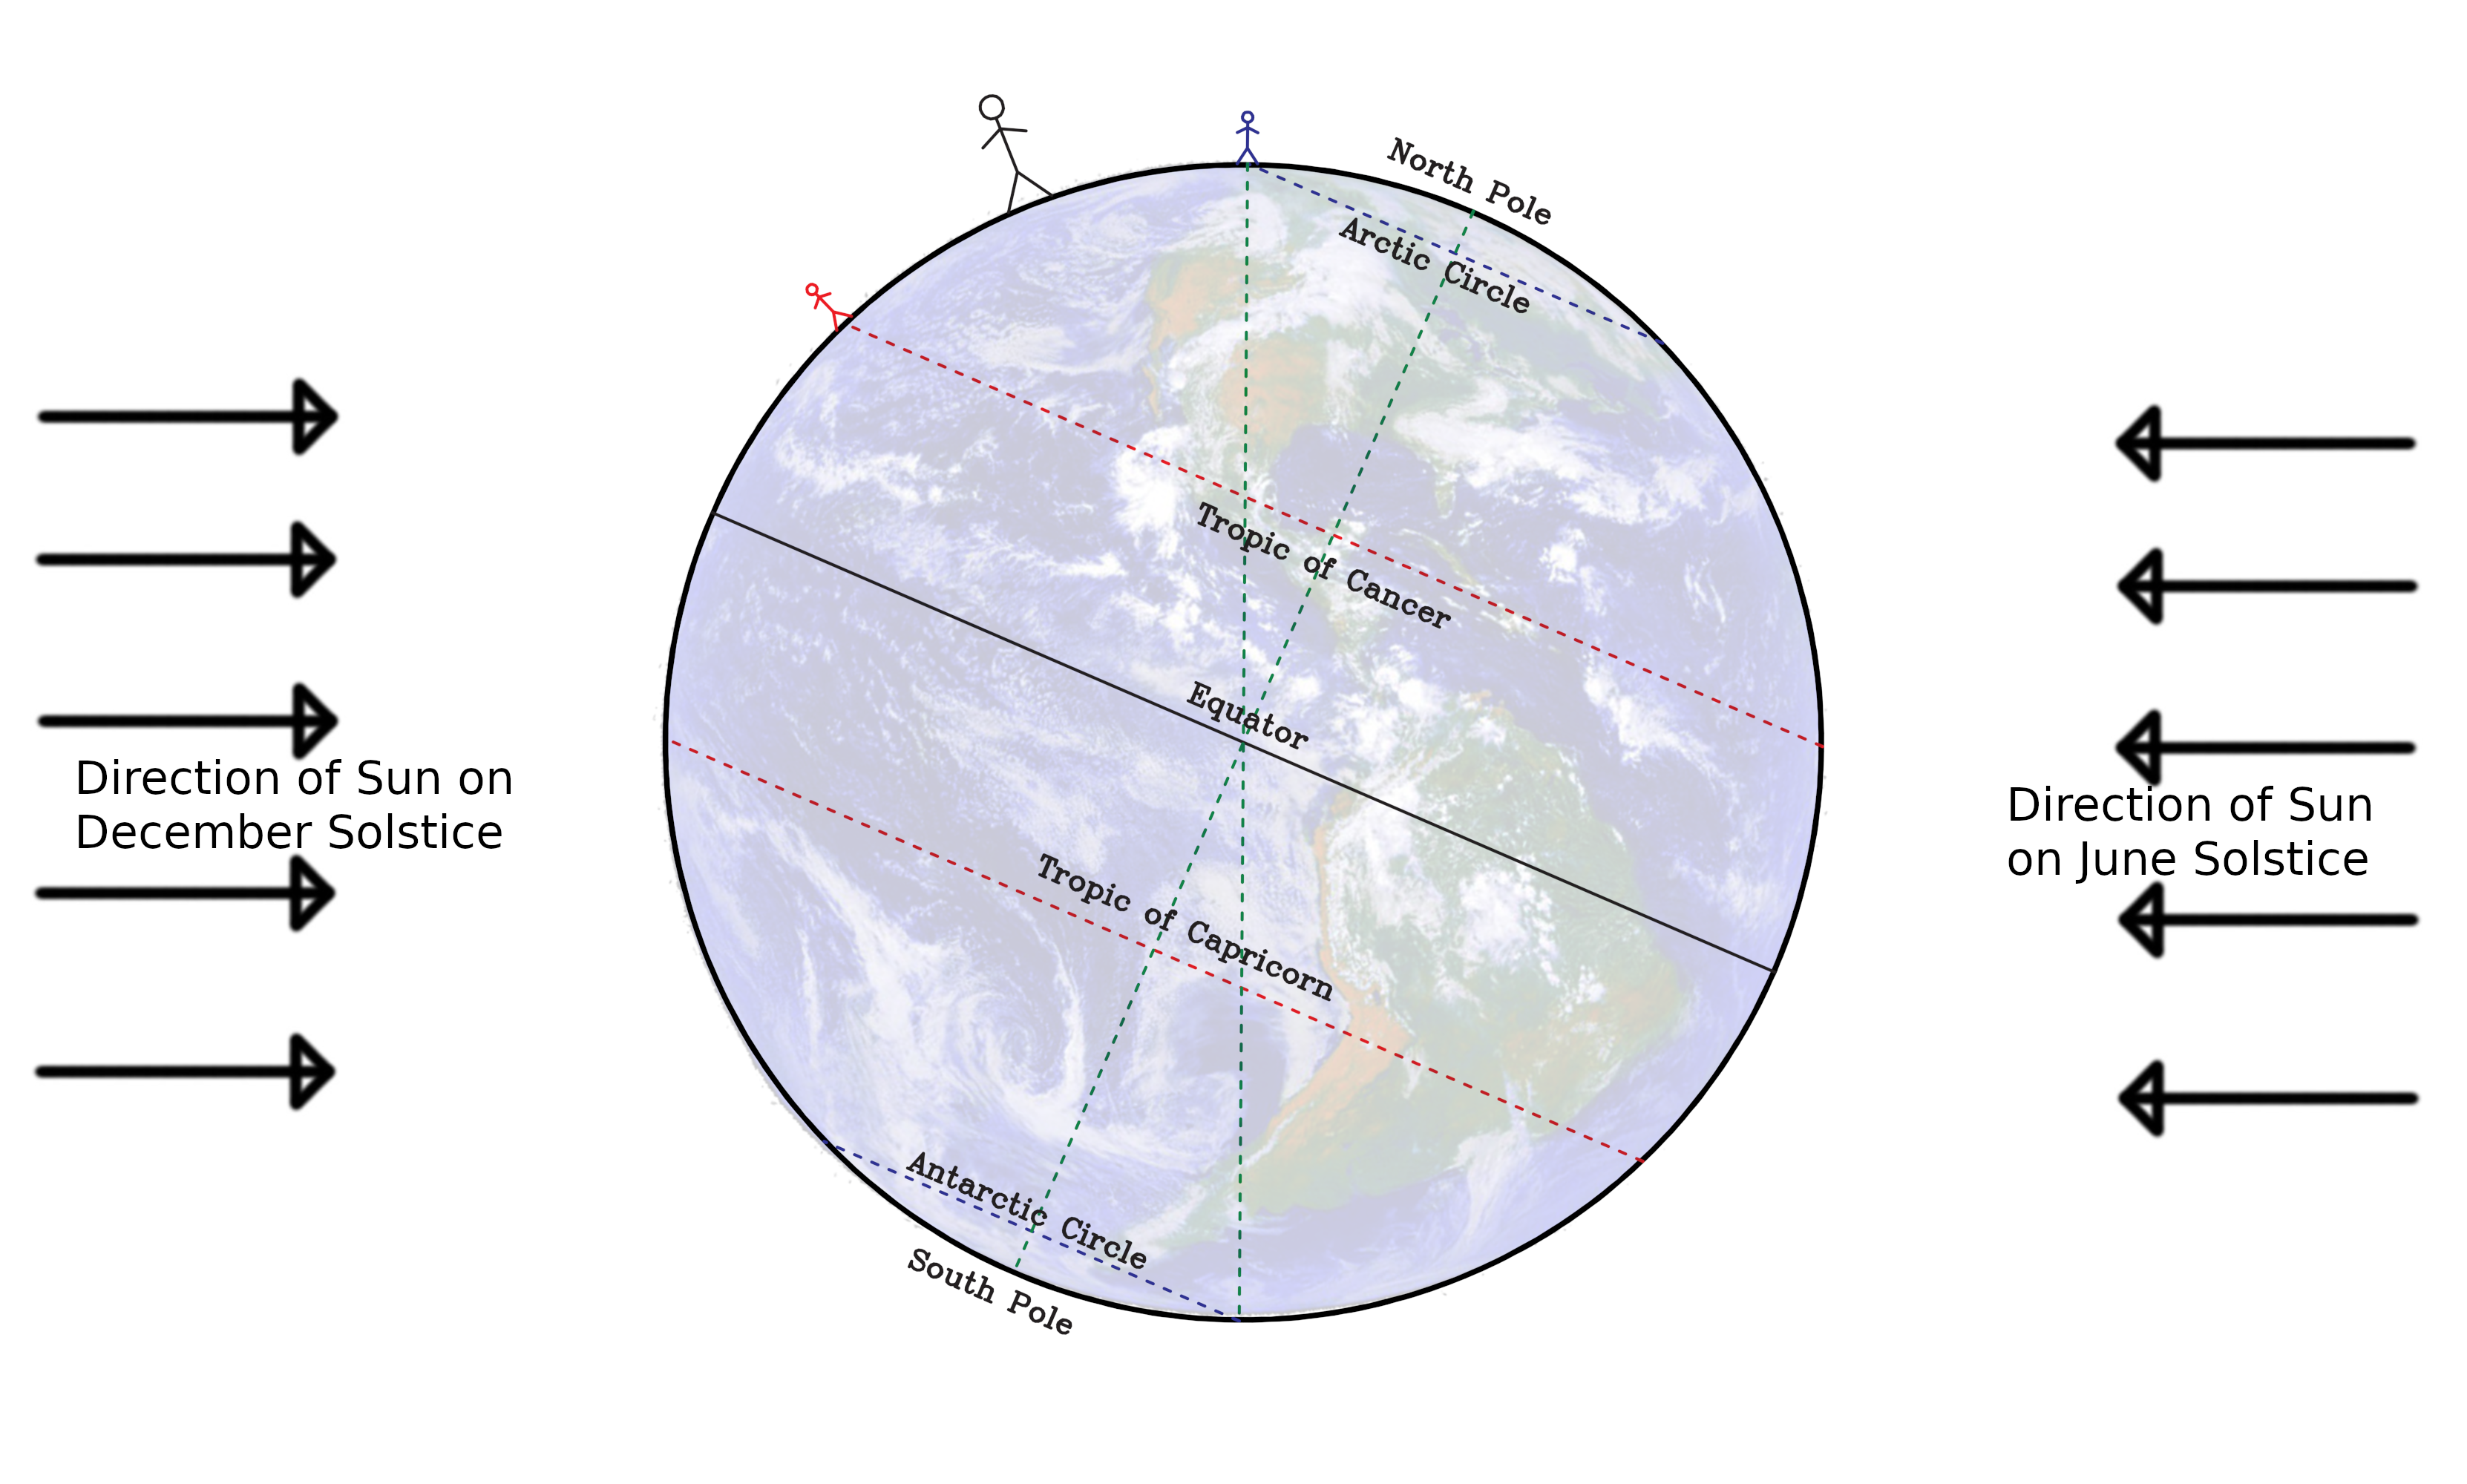
\includegraphics[width=10in]{earth-diagram-both.png}
	

	
\end{landscape}

	


\end{document}


